\author{Yuri}
For this project, we have decided to allow communication between STM32F407 and Arduino board trough two HC-05 modules.\\
HC-05 module is an easy to use Bluetooth SPP (Serial Port Protocol) module, designed for transparent wireless serial connection setup. The HC-05 Bluetooth Module can be used in a Master or Slave configuration, making it a great solution for wireless communication.\\

\begin{figure}[H]
	\centering
	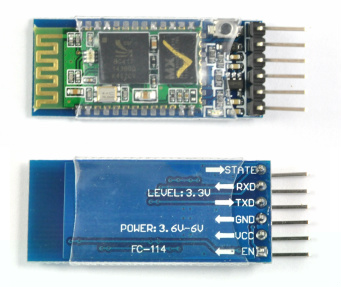
\includegraphics[width=\textwidth]
	{files/images/hc05_view}
	\caption{View of the surfaces of the HC-05 module.}
\end{figure}

\subsection{COMMAND and DATA TRANSFER MODES}
The module has two modes of operation: Command Mode where we can send AT commands to it, and Data Mode where it transmits and receives data to another Bluetooth module.\\

\textbf{Default Settings}\\
The default settings for new modules are
\begin{itemize}
\item Name = HC-05
\item Password = 1234
\item Baud rate in communication mode = 9600*
\item Baud rate in AT/Command mode = 38400
\end{itemize}

*sometimes 38400\\

The default mode is DATA Mode, and it is used to transmit data over Bluetooth communication.\\
AT command mode allows you to interrogate the Bluetooth module and to change some of the settings: like the name, the baud rate, whether or not it operates in slave mode or master mode.\\
When used as a master device AT commands allow you to connect to other Bluetooth slave devices.\\
For the project, we need to change some of the configuration setup values in AT command mode. \\

There are two ways to operate in Command Mode: using a USB to TTL adapter, or using an Arduino board.\\
Link the HC-05 following this scheme (don’t plug +5V pin for now)\\

\begin{tabular}{|c|c|c|}
	\hline 
	\textbf{HC-05 pin} & \textbf{Connected to \textit{USB to TTL}} & \textbf{Or connected to \textit{Arduino}} \\ 
	\hline 
	(1) +5V & Vcc & Vcc \\ 
	\hline 
	(2) GND & GND & GND \\ 
	\hline 
	(3) Tx & Rx & Rx \\ 
	\hline 
	(4) Rx & Tx & Tx \\ 
	\hline 
\end{tabular} 

\subsubsection{How to enter command mode if your HC-05 has KEY pin}
\begin{tabular}{|c|c|c|}
	\hline 
	\textbf{HC-05 pin} & \textbf{Connected to \textit{USB to TTL}} & \textbf{Or connected to \textit{Arduino}} \\ 
	\hline 
	Key & Vcc & 3.3V \\ 
	\hline 
\end{tabular} \\

KEY: This pin has to be pulled high to enter AT mode.

\subsubsection{How to enter command mode if your HC-05 has EN pin instead of KEY pin}
\begin{figure}[H]
	\centering
	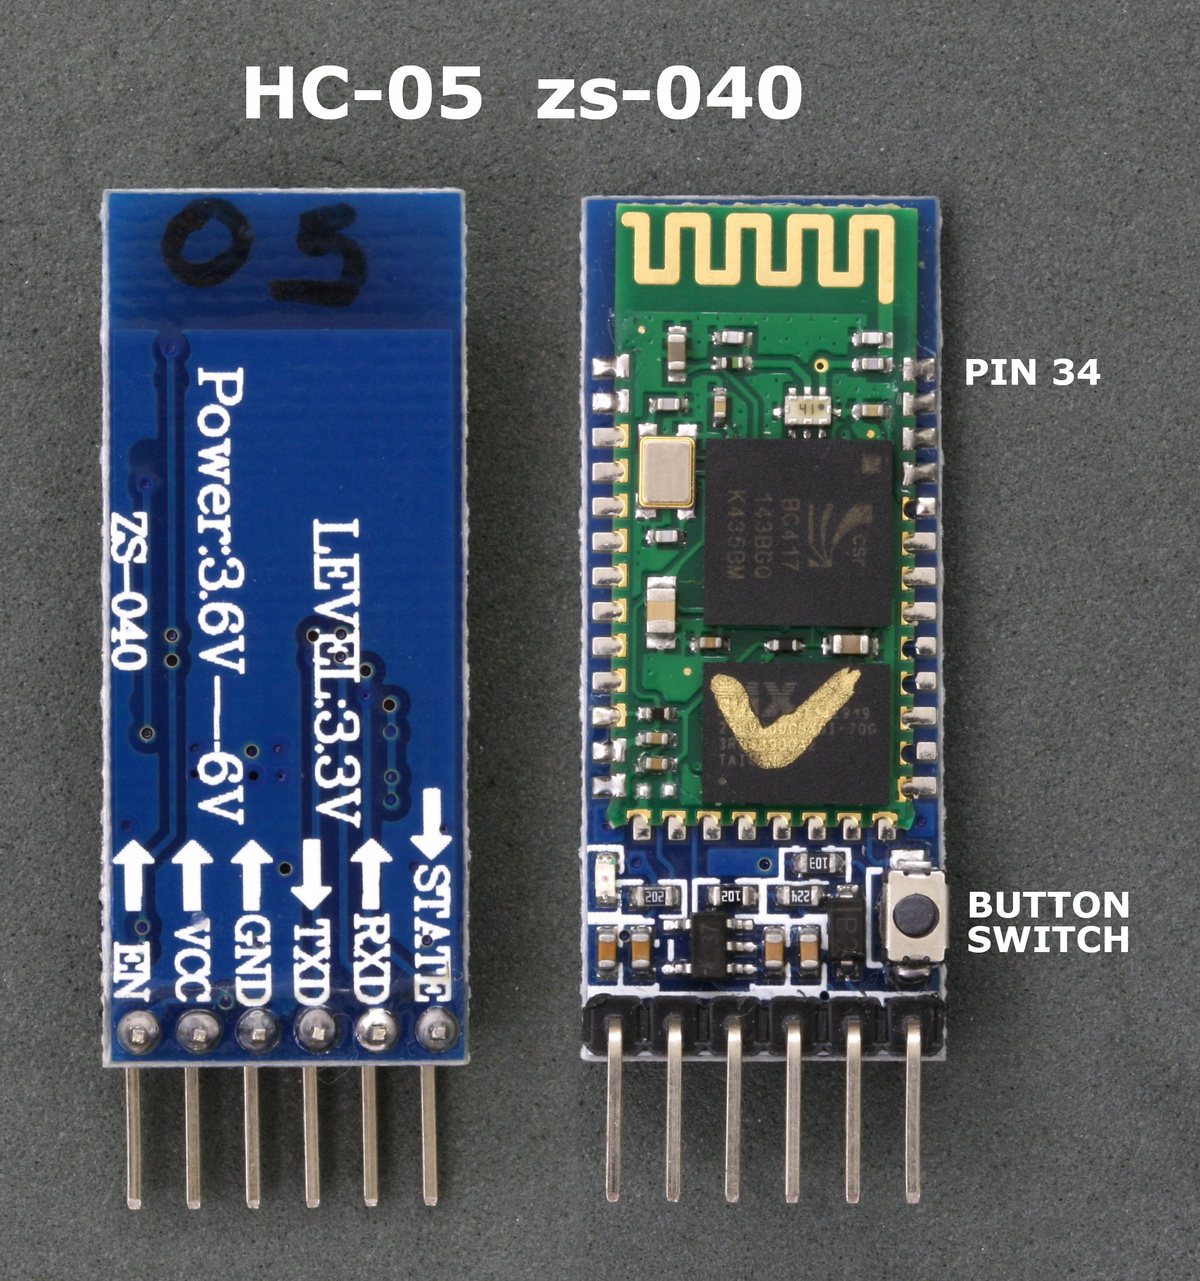
\includegraphics[width=\textwidth]
	{files/images/hc05_en_pin}
	\caption{HC-05 module with EN pin and switch button.}
\end{figure}
To activate AT mode on these HC-05 modules, pin 34 needs to be HIGH on power up. The small push button switch connects pin 34 to +3.3v so we can either:
\begin{itemize}
	\item connect pin 34 directly to +3v3v and power on, or
	\item hold the button switch closed when starting the module.
	
\end{itemize}
\textbf{METHOD 1} - Using the button switch to enter AT command mode:
\begin{enumerate}
	\item remove power from the module
	\item hold the small button switch closed while powering on the module.
	\item press and hold the button switch.
	\item while still holding the button switch closed, apply power.
	\item when you see the LED come on you can release the button switch.
\end{enumerate}
If the Bluetooth module led is flashing every 2 seconds (slower than usual) that means that we have successfully entered in the AT command mode.\\
\textbf{METHOD 2} - Using pin 34 to enter full AT command mode:
\begin{enumerate}
	\item remove power from the module
	\item make a connection between pin 34 and +3.3v
	\item reapply power.
\end{enumerate}
\begin{figure}[H]
	\centering
	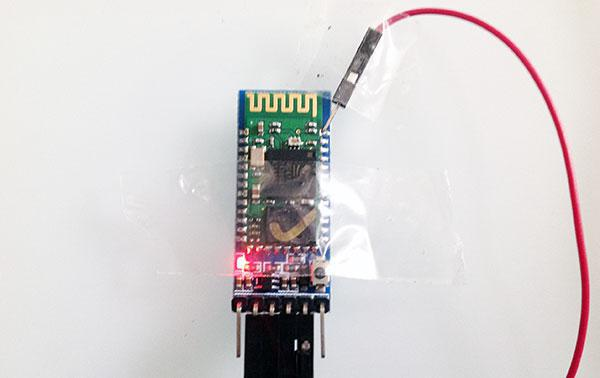
\includegraphics[width=\textwidth]
	{files/images/hc05_pin34}
	\caption{Example of connection bewteen pin 34 and +3.3v.}
\end{figure}
If the Bluetooth module led is flashing every 2 seconds (slower than usual) that means that we have successfully entered in the AT command mode.

\subsection{Setup the communication}
Final scheme:
STM32F407 -> HC-05 (master)    -->bluetooth communication<--    HC-05 (slave) <- Arduino

Once the HC-05 is in Command mode, we can use \textit{“Arduino Serial Monitor”} to set the HC-05 module.\\
After we run the Serial Monitor, we need to select \textit{“Both NL and CR”}, as well as, \textit{“38400 baud”} which is the default baud rate in command mode. Now, we are ready to send commands.\\

\subsection{HOW TO PAIR THE TWO MODULES}

\subsubsection{Slave configuration (this HC-05 module will be used on the Arduino Board)}
If we type just \textit{“AT”} which is a test command we should get back the message \textit{“OK”}.\\
Then if we type \textit{“AT+UART?”} we should get back the massage that shows the default baud rate which is \textit{9600}. (\textbf{REMEMBER, we will use the same baud rate on the Arduino board)}\\
Then if we type \textit{“AT+ROLE?”} we will get back a massage \textit{“+ROLE=0”} which means that the Bluetooth device is in slave mode. If we type \textit{“AT+ADDR?”} we will get back the address of the Bluetooth module and it should looks something like this: 18:e4:34cldd. \\
Now we need to write down this address, as we will need it when configuring the master device.
\begin{figure}[H]
	\centering
	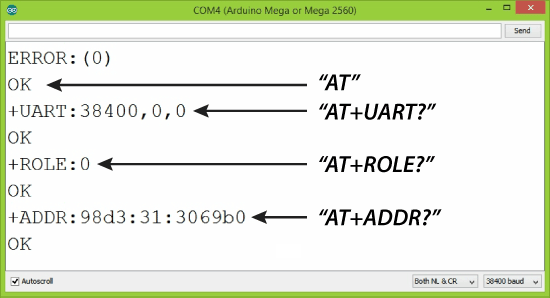
\includegraphics[width=\textwidth]
	{files/images/hc05_slave2}
	\caption{Slave configuration of the HC-05 module trough serial monitor.}
\end{figure}

\subsubsection{Master configuration (this HC-05 module will be used on the STM32F407 Discovery Board)}
The STM32F407 uses \textit{19200} baud rate to communicate on USART2, so we need to change the hc-05 baud rate, in addition to pair the master with his slave.\\
To speedup the baudrate to \textit{19200 bauds}, we have to type \textit{“AT+UART=19200,0,0”}.\\
Then by typing \textit{“AT+ROLE=1”} we will set the Bluetooth module as a master device. After this using the \textit{“AT+CMODE=0”} we will set the connect mode to “fixed address” and using the \textit{“AT+BIND=XX,XXXX,XX”} command we will set the address of the slave device that we previously wrote down.\\ \textbf{(Use commas, instead of colons!)}\\
\textit{“AT+BIND=18,e4,34cldd”} in our case.\\
\begin{figure}[H]
	\centering
	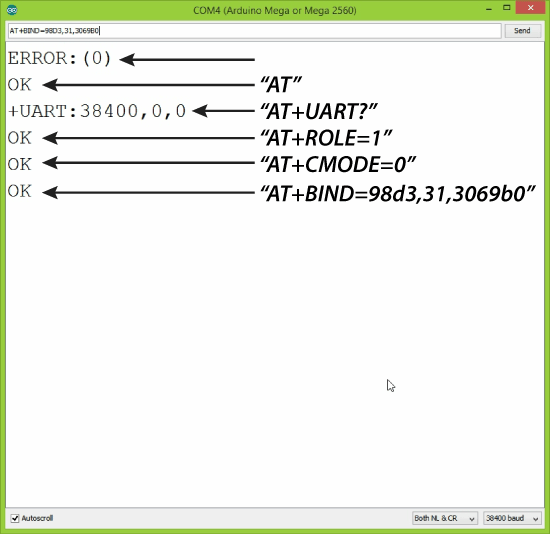
\includegraphics[width=\textwidth]
	{files/images/hc05_master}
	\caption{Master configuration of the HC-05 module trough serial monitor.}
\end{figure}
 
\subsection{STM32F407 CODE (Transmitter)}
The code loaded on the STM32F407 uses the USART2 channel to communicate with the HC-05 module.\\
So, we should link the HC-05 Rx pin to \textbf{PA2 pin (USART2 TX)} and HC-05 Tx pin to \textbf{PA3 (USART2 RX)}\\
In our project, we only send strings from SMT32F407 to Arduino (not vice versa), so the code will only write on the PA2 pin. (It is not necessary to link HC-05 Tx to PA3 pin for our purpose)\\
To send a string, we just need to use the “printf” function implemented in the miosix kernel.\\
\subsection{ARDUINO CODE (Receiver)}
\textit{“ArduinoBluetoothTest.txt”} contains a sketch with allow us to send and receive strings trough Bluetooth communication.\\
We decided to use \textbf{PIN 12 (TX)} and \textbf{PIN 11 (RX)} to communicate with the HC-05 module.\\
So, we should link the HC-05 Rx pin to PIN 12 and HC-05 Tx pin to PIN 11.\\
In our project we only send strings from SMT32F407 to Arduino (not vice versa), so the code will only read from PIN 11. (It’s not necessary to link HC-05 Rx to PIN 12 pin for our purpose)\\
To read a string from the HC-05 on Arduino is enough to use the \textit{read()} function of the SoftwareSerial class.\\